% Options for packages loaded elsewhere
\PassOptionsToPackage{unicode}{hyperref}
\PassOptionsToPackage{hyphens}{url}
%
\documentclass[
  11pt,
]{article}
\usepackage{amsmath,amssymb}
\usepackage{lmodern}
\usepackage{iftex}
\ifPDFTeX
  \usepackage[T1]{fontenc}
  \usepackage[utf8]{inputenc}
  \usepackage{textcomp} % provide euro and other symbols
\else % if luatex or xetex
  \usepackage{unicode-math}
  \defaultfontfeatures{Scale=MatchLowercase}
  \defaultfontfeatures[\rmfamily]{Ligatures=TeX,Scale=1}
\fi
% Use upquote if available, for straight quotes in verbatim environments
\IfFileExists{upquote.sty}{\usepackage{upquote}}{}
\IfFileExists{microtype.sty}{% use microtype if available
  \usepackage[]{microtype}
  \UseMicrotypeSet[protrusion]{basicmath} % disable protrusion for tt fonts
}{}
\makeatletter
\@ifundefined{KOMAClassName}{% if non-KOMA class
  \IfFileExists{parskip.sty}{%
    \usepackage{parskip}
  }{% else
    \setlength{\parindent}{0pt}
    \setlength{\parskip}{6pt plus 2pt minus 1pt}}
}{% if KOMA class
  \KOMAoptions{parskip=half}}
\makeatother
\usepackage{xcolor}
\usepackage[margin=1in]{geometry}
\usepackage{color}
\usepackage{fancyvrb}
\newcommand{\VerbBar}{|}
\newcommand{\VERB}{\Verb[commandchars=\\\{\}]}
\DefineVerbatimEnvironment{Highlighting}{Verbatim}{commandchars=\\\{\}}
% Add ',fontsize=\small' for more characters per line
\usepackage{framed}
\definecolor{shadecolor}{RGB}{248,248,248}
\newenvironment{Shaded}{\begin{snugshade}}{\end{snugshade}}
\newcommand{\AlertTok}[1]{\textcolor[rgb]{0.94,0.16,0.16}{#1}}
\newcommand{\AnnotationTok}[1]{\textcolor[rgb]{0.56,0.35,0.01}{\textbf{\textit{#1}}}}
\newcommand{\AttributeTok}[1]{\textcolor[rgb]{0.77,0.63,0.00}{#1}}
\newcommand{\BaseNTok}[1]{\textcolor[rgb]{0.00,0.00,0.81}{#1}}
\newcommand{\BuiltInTok}[1]{#1}
\newcommand{\CharTok}[1]{\textcolor[rgb]{0.31,0.60,0.02}{#1}}
\newcommand{\CommentTok}[1]{\textcolor[rgb]{0.56,0.35,0.01}{\textit{#1}}}
\newcommand{\CommentVarTok}[1]{\textcolor[rgb]{0.56,0.35,0.01}{\textbf{\textit{#1}}}}
\newcommand{\ConstantTok}[1]{\textcolor[rgb]{0.00,0.00,0.00}{#1}}
\newcommand{\ControlFlowTok}[1]{\textcolor[rgb]{0.13,0.29,0.53}{\textbf{#1}}}
\newcommand{\DataTypeTok}[1]{\textcolor[rgb]{0.13,0.29,0.53}{#1}}
\newcommand{\DecValTok}[1]{\textcolor[rgb]{0.00,0.00,0.81}{#1}}
\newcommand{\DocumentationTok}[1]{\textcolor[rgb]{0.56,0.35,0.01}{\textbf{\textit{#1}}}}
\newcommand{\ErrorTok}[1]{\textcolor[rgb]{0.64,0.00,0.00}{\textbf{#1}}}
\newcommand{\ExtensionTok}[1]{#1}
\newcommand{\FloatTok}[1]{\textcolor[rgb]{0.00,0.00,0.81}{#1}}
\newcommand{\FunctionTok}[1]{\textcolor[rgb]{0.00,0.00,0.00}{#1}}
\newcommand{\ImportTok}[1]{#1}
\newcommand{\InformationTok}[1]{\textcolor[rgb]{0.56,0.35,0.01}{\textbf{\textit{#1}}}}
\newcommand{\KeywordTok}[1]{\textcolor[rgb]{0.13,0.29,0.53}{\textbf{#1}}}
\newcommand{\NormalTok}[1]{#1}
\newcommand{\OperatorTok}[1]{\textcolor[rgb]{0.81,0.36,0.00}{\textbf{#1}}}
\newcommand{\OtherTok}[1]{\textcolor[rgb]{0.56,0.35,0.01}{#1}}
\newcommand{\PreprocessorTok}[1]{\textcolor[rgb]{0.56,0.35,0.01}{\textit{#1}}}
\newcommand{\RegionMarkerTok}[1]{#1}
\newcommand{\SpecialCharTok}[1]{\textcolor[rgb]{0.00,0.00,0.00}{#1}}
\newcommand{\SpecialStringTok}[1]{\textcolor[rgb]{0.31,0.60,0.02}{#1}}
\newcommand{\StringTok}[1]{\textcolor[rgb]{0.31,0.60,0.02}{#1}}
\newcommand{\VariableTok}[1]{\textcolor[rgb]{0.00,0.00,0.00}{#1}}
\newcommand{\VerbatimStringTok}[1]{\textcolor[rgb]{0.31,0.60,0.02}{#1}}
\newcommand{\WarningTok}[1]{\textcolor[rgb]{0.56,0.35,0.01}{\textbf{\textit{#1}}}}
\usepackage{longtable,booktabs,array}
\usepackage{calc} % for calculating minipage widths
% Correct order of tables after \paragraph or \subparagraph
\usepackage{etoolbox}
\makeatletter
\patchcmd\longtable{\par}{\if@noskipsec\mbox{}\fi\par}{}{}
\makeatother
% Allow footnotes in longtable head/foot
\IfFileExists{footnotehyper.sty}{\usepackage{footnotehyper}}{\usepackage{footnote}}
\makesavenoteenv{longtable}
\usepackage{graphicx}
\makeatletter
\def\maxwidth{\ifdim\Gin@nat@width>\linewidth\linewidth\else\Gin@nat@width\fi}
\def\maxheight{\ifdim\Gin@nat@height>\textheight\textheight\else\Gin@nat@height\fi}
\makeatother
% Scale images if necessary, so that they will not overflow the page
% margins by default, and it is still possible to overwrite the defaults
% using explicit options in \includegraphics[width, height, ...]{}
\setkeys{Gin}{width=\maxwidth,height=\maxheight,keepaspectratio}
% Set default figure placement to htbp
\makeatletter
\def\fps@figure{htbp}
\makeatother
\setlength{\emergencystretch}{3em} % prevent overfull lines
\providecommand{\tightlist}{%
  \setlength{\itemsep}{0pt}\setlength{\parskip}{0pt}}
\setcounter{secnumdepth}{-\maxdimen} % remove section numbering
\usepackage{hyperref}
\usepackage{array}
\usepackage{caption}
\usepackage{graphicx}
\usepackage{multirow}
\usepackage{hhline}
\usepackage{calc}
\usepackage{tabularx}
\usepackage[para,online,flushleft]{threeparttable}
\ifLuaTeX
  \usepackage{selnolig}  % disable illegal ligatures
\fi
\IfFileExists{bookmark.sty}{\usepackage{bookmark}}{\usepackage{hyperref}}
\IfFileExists{xurl.sty}{\usepackage{xurl}}{} % add URL line breaks if available
\urlstyle{same} % disable monospaced font for URLs
\hypersetup{
  pdftitle={Analysis of Health Survey for England (HSE) 2019},
  pdfauthor={Candidate Numbers Here},
  hidelinks,
  pdfcreator={LaTeX via pandoc}}

\title{Analysis of Health Survey for England (HSE) 2019}
\author{Candidate Numbers Here}
\date{March 08, 2024}

\begin{document}
\maketitle
\begin{abstract}
This report provides an analysis of data related to health, age,
socio-economic factors and lifestyle habits in adults (from the age of
16) from the population in England, derived from the Health Survey for
England 2019.
\end{abstract}

\newpage

\hypertarget{introduction}{%
\section{Introduction}\label{introduction}}

This is a body of text. \emph{This is an italic body of text.}
\href{https://google.com}{This is a clickable link!}.

\hypertarget{some-yaml-stuff}{%
\section{Some YAML Stuff}\label{some-yaml-stuff}}

The lion's share of a R Markdown document will be raw text, though the
front matter may be the most important part of the document. R Markdown
uses \href{http://www.yaml.org/}{YAML} for its metadata and the fields
differ from
\href{http://svmiller.com/blog/2015/02/moving-from-beamer-to-r-markdown/}{what
an author would use for a Beamer presentation}. I provide a sample YAML
metadata largely taken from this exact document and explain it below.

\begin{Shaded}
\begin{Highlighting}[]
\SpecialCharTok{{-}{-}{-}}
\NormalTok{output}\SpecialCharTok{:} 
\NormalTok{  pdf\_document}\SpecialCharTok{:}
\NormalTok{    keep\_tex}\SpecialCharTok{:}\NormalTok{ true}
\NormalTok{    fig\_caption}\SpecialCharTok{:}\NormalTok{ true}
\NormalTok{    latex\_engine}\SpecialCharTok{:}\NormalTok{ pdflatex}
\NormalTok{title}\SpecialCharTok{:} \StringTok{"A Pandoc Markdown Article Starter and Template"}
\NormalTok{abstract}\SpecialCharTok{:} \StringTok{"This document provides an introduction to R Markdown, argues for its..."}
\NormalTok{date}\SpecialCharTok{:} \StringTok{"\textasciigrave{}r format(Sys.time(), \textquotesingle{}\%B \%d, \%Y\textquotesingle{})\textasciigrave{}"}
\NormalTok{geometry}\SpecialCharTok{:}\NormalTok{ margin}\OtherTok{=}\NormalTok{1in}
\NormalTok{fontsize}\SpecialCharTok{:}\NormalTok{ 11pt}
\CommentTok{\# spacing: double}
\SpecialCharTok{{-}{-}{-}}
\end{Highlighting}
\end{Shaded}

\texttt{output:} will tell R Markdown we want a PDF document rendered
with LaTeX. Since we are adding a fair bit of custom options to this
call, we specify \texttt{pdf\_document:} on the next line (with,
importantly, a two-space indent). We specify additional output-level
options underneath it, each are indented with four spaces. The line
(\texttt{keep\_tex:\ true}) tells R Markdown to render a raw
\texttt{.tex} file along with the PDF document. This is useful for both
debugging and the publication stage. The next line
\texttt{fig\_caption:\ true} tells R Markdown to make sure that whatever
images are included in the document are treated as figures in which our
caption in brackets in a Markdown call is treated as the caption in the
figure. The next line (\texttt{latex\_engine:\ pdflatex}) tells R
Markdown to use pdflatex and not some other option like
\texttt{lualatex}. For this template, I'm pretty sure this is
mandatory.{[}\^{}pdflatex{]}

The next fields get to the heart of the document itself. \texttt{title:}
is, intuitively, the title of the manuscript. Do note that fields like
\texttt{title:} do not have to be in quotation marks, but must be in
quotation marks if the title of the document includes a colon. That
said, the only reason to use a colon in an article title is if it is
followed by a subtitle, hence the optional field (\texttt{subtitle:}).
Notice I ``comment out'' the subtitle in the above example with a pound
sign since this particular document does not have a subtitle.

\texttt{date} comes standard with R Markdown and you can use it to enter
the date of the most recent compile.

The next items are optional and cosmetic. \texttt{geometry:} is a
standard option in LaTeX. I set the margins at one inch, and you
probably should too. \texttt{fontsize:} sets, intuitively, the font
size. The default is 10-point, but I prefer 11-point. \texttt{spacing:}
is an optional field. If it is set as ``double'', the ensuing document
is double-spaced. ``single'' is the only other valid entry for this
field, though not including the entry in the YAML metadata amounts to
singlespacing the document by default. Notice I have this ``commented
out'' in the example code.

\hypertarget{getting-started-with-markdown-syntax}{%
\section{Getting Started with Markdown
Syntax}\label{getting-started-with-markdown-syntax}}

There are a lot of cheatsheets and reference guides for Markdown
(e.g.~\href{https://github.com/adam-p/markdown-here/wiki/Markdown-Cheatsheet}{Adam
Prichard},
\href{http://assemble.io/docs/Cheatsheet-Markdown.html}{Assemble},
\href{https://www.rstudio.com/wp-content/uploads/2015/02/rmarkdown-cheatsheet.pdf}{Rstudio},
\href{https://www.rstudio.com/wp-content/uploads/2015/03/rmarkdown-reference.pdf}{Rstudio
again},
\href{http://scottboms.com/downloads/documentation/markdown_cheatsheet.pdf}{Scott
Boms}, \href{https://daringfireball.net/projects/markdown/syntax}{Daring
Fireball}, among, I'm sure, several others).

\begin{Shaded}
\begin{Highlighting}[]
\FunctionTok{\# Introduction}

\NormalTok{**Lorem ipsum** dolor *sit amet*. }

\SpecialStringTok{{-} }\NormalTok{Single asterisks italicize text *like this*. }
\SpecialStringTok{{-} }\NormalTok{Double asterisks embolden text **like this**.}

\NormalTok{Start a new paragraph with a blank line separating paragraphs.}

\SpecialStringTok{{-} }\NormalTok{This will start an unordered list environment, and this will be the first item.}
\SpecialStringTok{{-} }\NormalTok{This will be a second item.}
\SpecialStringTok{{-} }\NormalTok{A third item.}
\SpecialStringTok{    {-} }\NormalTok{Four spaces and a dash create a sublist and this item in it.}
\SpecialStringTok{{-} }\NormalTok{The fourth item.}
    
\SpecialStringTok{1. }\NormalTok{This starts a numerical list.}
\SpecialStringTok{2. }\NormalTok{This is no. 2 in the numerical list.}
    
\FunctionTok{\# This Starts A New Section}
\FunctionTok{\#\# This is a Subsection}
\FunctionTok{\#\#\# This is a Subsubsection}
\FunctionTok{\#\#\#\# This starts a Paragraph Block.}

\AttributeTok{\textgreater{} This will create a block quote, if you want one.}

\NormalTok{Want a table? This will create one.}

\NormalTok{Table Header  | Second Header}
\NormalTok{{-}{-}{-}{-}{-}{-}{-}{-}{-}{-}{-}{-}{-} | {-}{-}{-}{-}{-}{-}{-}{-}{-}{-}{-}{-}{-}}
\NormalTok{Table Cell    | Cell 2}
\NormalTok{Cell 3        | Cell 4 }

\NormalTok{Note that the separators *do not* have to be aligned.}

\NormalTok{Want an image? This will do it.}

\AlertTok{![caption for my image](path/to/image.jpg)}

\InformationTok{\textasciigrave{}fig\_caption: yes\textasciigrave{}}\NormalTok{ will provide a caption. Put that in the YAML metadata.}

\NormalTok{Almost forgot about creating a footnote.}\OtherTok{[\^{}1]}\NormalTok{ This will do it again.}\OtherTok{[\^{}2]}

\OtherTok{[\^{}1]: }\NormalTok{The first footnote}
\OtherTok{[\^{}2]: }\NormalTok{The second footnote}

\NormalTok{Want to cite something? }

\SpecialStringTok{{-} }\NormalTok{Find your biblatexkey in your bib file.}
\SpecialStringTok{{-} }\NormalTok{Put an @ before it, like @smith1984, or whatever it is.}
\SpecialStringTok{{-} }\NormalTok{@smith1984 creates an in{-}text citation (e.g. Smith (1984) says...)}
\SpecialStringTok{{-} }\CommentTok{[}\OtherTok{@smith1984}\CommentTok{]}\NormalTok{ creates a parenthetical citation (Smith, 1984)}

\NormalTok{That\textquotesingle{}ll also automatically create a reference list at the end of the document.}

\CommentTok{[}\OtherTok{In{-}text link to Google}\CommentTok{](http://google.com)}\NormalTok{ as well.}
\end{Highlighting}
\end{Shaded}

\hypertarget{checking-for-potential-data-issues}{%
\section{Checking for Potential Data
Issues}\label{checking-for-potential-data-issues}}

\hypertarget{handling-of-missing-values}{%
\subsection{Handling of Missing
Values}\label{handling-of-missing-values}}

The approach for handling missing values is as follows:

\begin{enumerate}
\def\labelenumi{\arabic{enumi}.}
\tightlist
\item
  If an entire row of descriptive variables is empty, the entire record
  can be deleted.
\item
  If key variables are missing, the entire record can be deleted. Key
  variables include \textbf{serialA}, \textbf{sex}, \textbf{Age35g10 OR
  ag16g10}, \textbf{cigdyal\_19 OR cigsta3\_19 OR NDPNow\_19}.
\item
  If a variable value is completely implausible (not just an outlier),
  it should be coded as missing, unless the true value is obvious.
\item
  If all variable values are outside the study population, the whole
  variable can be removed.
\item
  If all variable values are empty, the whole variable can be removed.
\item
  Missing values (codes, text) should all be recoded to the standard R
  value of `NA'.
\end{enumerate}

I perform these checks on our full dataset.

Firstly, we note that the study population is \emph{adults from the
population of England}, meaning that any records with an age group not
containing values of 16 years or higher must be excluded (if the age
group is missing for both variables, we assume they are under 16).

\begin{Shaded}
\begin{Highlighting}[]
\FunctionTok{library}\NormalTok{(haven) }\CommentTok{\# Required to present the summary of labelled data.}
\FunctionTok{library}\NormalTok{(dplyr) }\CommentTok{\# Required to use the pipe operator \%\textgreater{}\%.}
\FunctionTok{load}\NormalTok{(}\StringTok{"\textasciitilde{}/MA30091/Coursework/MA30091/Datasets/hsesub.Rdata"}\NormalTok{) }\CommentTok{\# The dset is called subdat.}
\CommentTok{\# I have checked, and the two age category variables match up.}
\NormalTok{subdat }\OtherTok{=} \FunctionTok{data.frame}\NormalTok{(subdat)}
\NormalTok{sd16plus }\OtherTok{\textless{}{-}}\NormalTok{ subdat }\SpecialCharTok{\%\textgreater{}\%}
  \FunctionTok{filter}\NormalTok{(ag16g10 }\SpecialCharTok{\textgreater{}=} \DecValTok{1} \SpecialCharTok{\&}\NormalTok{ Age35g }\SpecialCharTok{\textgreater{}=} \DecValTok{7} \SpecialCharTok{\&} \SpecialCharTok{!}\NormalTok{(}\FunctionTok{is.na}\NormalTok{(Age35g)}\SpecialCharTok{\&} \FunctionTok{is.na}\NormalTok{(ag16g10)))}
\CommentTok{\# As we are only dealing with adults, the ag16g10 variable is now the same as Age35g, except that it has lower resolution. As such, we can remove ag16g10.}
\NormalTok{sd16plusA }\OtherTok{=}\NormalTok{ sd16plus[,}\SpecialCharTok{{-}}\DecValTok{3}\NormalTok{]}
\FunctionTok{summary}\NormalTok{(sd16plusA)}
\end{Highlighting}
\end{Shaded}

\begin{verbatim}
##     SerialA             Sex            Age35g         wt_int      
##  Min.   :2900001   Min.   :1.000   Min.   : 7.0   Min.   :0.3155  
##  1st Qu.:2903106   1st Qu.:1.000   1st Qu.:11.0   1st Qu.:0.7914  
##  Median :2906225   Median :2.000   Median :14.0   Median :0.8828  
##  Mean   :2906233   Mean   :1.552   Mean   :13.8   Mean   :1.0000  
##  3rd Qu.:2909415   3rd Qu.:2.000   3rd Qu.:17.0   3rd Qu.:1.0785  
##  Max.   :2912463   Max.   :2.000   Max.   :22.0   Max.   :6.4927  
##                                                                   
##     topqual2        marstatD         qimd19         urban14b    
##  Min.   :1.000   Min.   :1.000   Min.   :1.000   Min.   :1.000  
##  1st Qu.:1.000   1st Qu.:2.000   1st Qu.:2.000   1st Qu.:1.000  
##  Median :3.000   Median :2.000   Median :3.000   Median :1.000  
##  Mean   :3.664   Mean   :2.658   Mean   :3.013   Mean   :1.188  
##  3rd Qu.:7.000   3rd Qu.:4.000   3rd Qu.:4.000   3rd Qu.:1.000  
##  Max.   :8.000   Max.   :6.000   Max.   :5.000   Max.   :2.000  
##  NA's   :46      NA's   :1                                      
##     origin2        cigsta3_19      cigdyal_19         BMIVal     
##  Min.   :1.000   Min.   :1.000   Min.   : 0.000   Min.   :14.53  
##  1st Qu.:1.000   1st Qu.:2.000   1st Qu.: 0.000   1st Qu.:23.92  
##  Median :1.000   Median :3.000   Median : 0.000   Median :27.06  
##  Mean   :1.288   Mean   :2.437   Mean   : 1.692   Mean   :27.87  
##  3rd Qu.:1.000   3rd Qu.:3.000   3rd Qu.: 0.000   3rd Qu.:30.86  
##  Max.   :5.000   Max.   :3.000   Max.   :60.000   Max.   :73.49  
##  NA's   :29      NA's   :56      NA's   :57       NA's   :1522   
##    NDPNow_19        dnoft_19       drinkYN_19      d7many3_19   
##  Min.   :1.000   Min.   :1.000   Min.   :1.000   Min.   :0.000  
##  1st Qu.:4.000   1st Qu.:3.000   1st Qu.:2.000   1st Qu.:0.000  
##  Median :4.000   Median :4.000   Median :2.000   Median :1.000  
##  Mean   :3.862   Mean   :4.281   Mean   :1.808   Mean   :1.594  
##  3rd Qu.:4.000   3rd Qu.:5.000   3rd Qu.:2.000   3rd Qu.:3.000  
##  Max.   :4.000   Max.   :8.000   Max.   :2.000   Max.   :7.000  
##  NA's   :53      NA's   :1499    NA's   :51      NA's   :52     
##     omsysval          GOR1      
##  Min.   : 75.0   Min.   :1.000  
##  1st Qu.:113.0   1st Qu.:3.000  
##  Median :123.5   Median :5.000  
##  Mean   :125.0   Mean   :5.155  
##  3rd Qu.:135.0   3rd Qu.:8.000  
##  Max.   :209.5   Max.   :9.000  
##  NA's   :4039
\end{verbatim}

\hypertarget{the-missing-adult}{%
\subsubsection{The Missing Adult}\label{the-missing-adult}}

The original brief tells us there are 8205 adults sampled, however our
dataset only contains 8204. In fact, the original dataset should contain
10300 observations, so we know that this is a data error. Perhaps this
patient did not have any data collected on them, or withdrew.

It is also worth mentioning that the below subset of 7144 adults are
only those who have at least one key physical measurement taken. We
proceed with the full dataset, but save this subset for later.

\begin{Shaded}
\begin{Highlighting}[]
\NormalTok{sdPhys }\OtherTok{\textless{}{-}}\NormalTok{ sd16plusA }\SpecialCharTok{\%\textgreater{}\%}
  \FunctionTok{filter}\NormalTok{(}\SpecialCharTok{!}\NormalTok{(}\FunctionTok{is.na}\NormalTok{(omsysval) }\SpecialCharTok{\&} \FunctionTok{is.na}\NormalTok{(BMIVal)))}
\FunctionTok{summary}\NormalTok{(sdPhys)}
\end{Highlighting}
\end{Shaded}

\begin{verbatim}
##     SerialA             Sex            Age35g          wt_int      
##  Min.   :2900001   Min.   :1.000   Min.   : 7.00   Min.   :0.3155  
##  1st Qu.:2903106   1st Qu.:1.000   1st Qu.:11.00   1st Qu.:0.7916  
##  Median :2906190   Median :2.000   Median :14.00   Median :0.8821  
##  Mean   :2906231   Mean   :1.552   Mean   :13.82   Mean   :1.0011  
##  3rd Qu.:2909425   3rd Qu.:2.000   3rd Qu.:17.00   3rd Qu.:1.0731  
##  Max.   :2912463   Max.   :2.000   Max.   :22.00   Max.   :6.4927  
##                                                                    
##     topqual2        marstatD        qimd19         urban14b        origin2     
##  Min.   :1.000   Min.   :1.00   Min.   :1.000   Min.   :1.000   Min.   :1.000  
##  1st Qu.:1.000   1st Qu.:2.00   1st Qu.:2.000   1st Qu.:1.000   1st Qu.:1.000  
##  Median :3.000   Median :2.00   Median :3.000   Median :1.000   Median :1.000  
##  Mean   :3.596   Mean   :2.65   Mean   :2.981   Mean   :1.191   Mean   :1.284  
##  3rd Qu.:6.000   3rd Qu.:4.00   3rd Qu.:4.000   3rd Qu.:1.000   3rd Qu.:1.000  
##  Max.   :8.000   Max.   :6.00   Max.   :5.000   Max.   :2.000   Max.   :5.000  
##  NA's   :20      NA's   :1                                      NA's   :5      
##    cigsta3_19      cigdyal_19         BMIVal        NDPNow_19    
##  Min.   :1.000   Min.   : 0.000   Min.   :14.53   Min.   :1.000  
##  1st Qu.:2.000   1st Qu.: 0.000   1st Qu.:23.92   1st Qu.:4.000  
##  Median :3.000   Median : 0.000   Median :27.06   Median :4.000  
##  Mean   :2.443   Mean   : 1.667   Mean   :27.87   Mean   :3.863  
##  3rd Qu.:3.000   3rd Qu.: 0.000   3rd Qu.:30.86   3rd Qu.:4.000  
##  Max.   :3.000   Max.   :60.000   Max.   :73.49   Max.   :4.000  
##  NA's   :18      NA's   :18       NA's   :462     NA's   :16     
##     dnoft_19       drinkYN_19     d7many3_19       omsysval          GOR1      
##  Min.   :1.000   Min.   :1.00   Min.   :0.000   Min.   : 75.0   Min.   :1.000  
##  1st Qu.:3.000   1st Qu.:2.00   1st Qu.:0.000   1st Qu.:113.0   1st Qu.:3.000  
##  Median :4.000   Median :2.00   Median :1.000   Median :123.5   Median :5.000  
##  Mean   :4.268   Mean   :1.82   Mean   :1.641   Mean   :125.0   Mean   :5.168  
##  3rd Qu.:5.000   3rd Qu.:2.00   3rd Qu.:3.000   3rd Qu.:135.0   3rd Qu.:8.000  
##  Max.   :8.000   Max.   :2.00   Max.   :7.000   Max.   :209.5   Max.   :9.000  
##  NA's   :1193    NA's   :15     NA's   :16      NA's   :2979
\end{verbatim}

\hypertarget{duplicate-entries}{%
\subsection{Duplicate Entries}\label{duplicate-entries}}

\begin{Shaded}
\begin{Highlighting}[]
\CommentTok{\# Firstly, we need to check that no ID variables are duplicated.}
\FunctionTok{anyDuplicated}\NormalTok{(sd16plusA}\SpecialCharTok{$}\NormalTok{SerialA)}
\end{Highlighting}
\end{Shaded}

\begin{verbatim}
## [1] FALSE
\end{verbatim}

\begin{Shaded}
\begin{Highlighting}[]
\CommentTok{\# There are none.}

\CommentTok{\# Now, we check whether we have any exact copies in all other variables (not including ID or any variables that could have been recorded as an accidental second visit like quantified questionnaire data or lab data).}
 
\NormalTok{dupesFront }\OtherTok{=} \FunctionTok{duplicated}\NormalTok{(sd16plusA[,}\SpecialCharTok{{-}}\FunctionTok{c}\NormalTok{(}\DecValTok{1}\NormalTok{, }\DecValTok{12}\NormalTok{, }\DecValTok{17}\NormalTok{)])}
\NormalTok{dupesBack }\OtherTok{=}  \FunctionTok{duplicated}\NormalTok{(sd16plusA[,}\SpecialCharTok{{-}}\FunctionTok{c}\NormalTok{(}\DecValTok{1}\NormalTok{, }\DecValTok{12}\NormalTok{, }\DecValTok{17}\NormalTok{)], }\AttributeTok{fromLast =} \ConstantTok{TRUE}\NormalTok{)}
\FunctionTok{which}\NormalTok{(dupesFront }\SpecialCharTok{==} \DecValTok{1} \SpecialCharTok{|}\NormalTok{ dupesBack }\SpecialCharTok{==} \DecValTok{1}\NormalTok{) }\CommentTok{\# This will output the indices of where duplicate observations occur *including the first occurrence*.}
\end{Highlighting}
\end{Shaded}

\begin{verbatim}
##  [1]  369  512 1191 1192 1248 1249 1250 1279 1280 1281 1334 1992 2056 2057 2813
## [16] 3022 3023 3062 3063 3174 3175 3492 4236 4639 4727 4752 4753 5268 5269 6314
## [31] 6316 6727 7287 7305 7359 7496 7497 7510 7516
\end{verbatim}

\begin{Shaded}
\begin{Highlighting}[]
\NormalTok{dupes2 }\OtherTok{=}\NormalTok{ sd16plusA[}\FunctionTok{which}\NormalTok{(dupesFront }\SpecialCharTok{==} \DecValTok{1} \SpecialCharTok{|}\NormalTok{ dupesBack }\SpecialCharTok{==} \DecValTok{1}\NormalTok{),}\SpecialCharTok{{-}}\DecValTok{1}\NormalTok{]}
\NormalTok{dupesFin }\OtherTok{\textless{}{-}}\NormalTok{ dupes2[}\FunctionTok{order}\NormalTok{(dupes2}\SpecialCharTok{$}\NormalTok{wt\_int),]}
\NormalTok{dupesFin}
\end{Highlighting}
\end{Shaded}

\begin{verbatim}
##      Sex Age35g    wt_int topqual2 marstatD qimd19 urban14b origin2 cigsta3_19
## 6727   1     17 0.8157590        4        2      1        2       1          3
## 7359   1     17 0.8157590        4        2      1        2       1          3
## 1250   2     16 0.8361538        4        4      4        1       1          2
## 4727   2     16 0.8361538        4        4      4        1       1          2
## 3062   2     21 0.8712937        7        5      2        1       1          3
## 3063   2     21 0.8712937        7        5      2        1       1          3
## 4752   2      8 0.8734320        1        1      3        1       3          3
## 4753   2      8 0.8734320        1        1      3        1       3          3
## 2813   2     21 0.8755313        7        5      3        2       1          3
## 3492   2     21 0.8755313        7        5      3        2       1          3
## 369    2     19 0.8765687        1        5      2        1       1          3
## 7305   2     19 0.8765687        1        5      2        1       1          3
## 4236   2     20 0.8906912        1        5      1        1       1          3
## 4639   2     20 0.8906912        1        5      1        1       1          3
## 1992   1     14 0.8934150        1        1      1        1       1          3
## 7287   1     14 0.8934150        1        1      1        1       1          3
## 1248   2      7 1.1020298        8        1      3        1       3          3
## 1249   2      7 1.1020298        8        1      3        1       3          3
## 3022   2      8 1.1509630        8        1      5        1       2          3
## 3023   2      8 1.1509630        8        1      5        1       2          3
## 7496   2      7 1.2011841        8        1      1        1       3          3
## 7497   2      7 1.2011841        8        1      1        1       3          3
## 7510   2      9 1.3199261        1        6      3        1       1          3
## 7516   2      9 1.3199261        1        6      3        1       1          3
## 1279   2      8 1.4034707        8        1      4        1       3          3
## 1280   2      8 1.4034707        8        1      4        1       3          3
## 1281   2      8 1.4034707        8        1      4        1       3          3
## 6314   2      8 1.5105870        8        1      2        1       1          3
## 6316   2      8 1.5105870        8        1      2        1       1          3
## 5268   2      8 1.5895207        8        1      5        1       2          3
## 5269   2      8 1.5895207        8        1      5        1       2          3
## 512    1      7 1.6111765        8        1      1        1       1          3
## 1334   1      7 1.6111765        8        1      1        1       1          3
## 2056   2      7 1.7317897        4        1      4        1       1          3
## 2057   2      7 1.7317897        4        1      4        1       1          3
## 1191   1      9 1.7556401        7        2      3        1       1          3
## 1192   1      9 1.7556401        7        2      3        1       1          3
## 3174   1      7 2.5196747        8        1      4        1       3          3
## 3175   1      7 2.5196747        8        1      4        1       3          3
##      cigdyal_19   BMIVal NDPNow_19 dnoft_19 drinkYN_19 d7many3_19 omsysval GOR1
## 6727          0 36.91150         4        6          2          0       NA    6
## 7359          0 31.16046         4        6          2          0    110.5    6
## 1250          0       NA         4       NA          1          0       NA    9
## 4727          0       NA         4       NA          1          0       NA    9
## 3062          0       NA         4       NA          1          0       NA    3
## 3063          0 25.81338         4       NA          1          0       NA    3
## 4752          0 21.79088         4        6          2          1     97.5    8
## 4753          0       NA         4        6          2          1     95.0    8
## 2813          0 24.98638         4       NA          1          0    164.0    6
## 3492          0 24.57274         4       NA          1          0    116.0    6
## 369           0       NA         4        7          2          0       NA    4
## 7305          0 27.41666         4        7          2          0    108.0    4
## 4236          0 22.59219         4       NA          1          0       NA    7
## 4639          0 21.42687         4       NA          1          0       NA    7
## 1992          0 26.36697         4       NA          1          0    119.0    8
## 7287          0 22.64334         4       NA          1          0    134.0    8
## 1248          0 22.27153         4       NA          1          0       NA    9
## 1249          0 25.59686         4       NA          1          0       NA    9
## 3022          0 22.64493         4       NA          1          0       NA    3
## 3023          0 22.04727         4       NA          1          0       NA    3
## 7496          0 19.80584         4       NA          1          0       NA    6
## 7497          0 18.83437         4       NA          1          0     92.5    6
## 7510          0 23.00056         4        4          2          2    107.5    7
## 7516          0 20.63814         4        4          2          2    115.0    7
## 1279          0       NA         4       NA          1          0       NA    8
## 1280          0       NA         4       NA          1          0       NA    8
## 1281          0       NA         4       NA          1          0    108.5    8
## 6314          0 18.46158         4        5          2          1    121.0    8
## 6316          0 26.67950         4        5          2          1    103.0    8
## 5268          0 19.94309         4       NA          1          0    102.5    7
## 5269          0 18.81037         4       NA          1          0       NA    7
## 512           0 21.81825         4        5          2          0    124.5    8
## 1334          0       NA         4        5          2          0       NA    8
## 2056          0 23.10065         4        4          2          2    116.0    7
## 2057          0 25.61760         4        4          2          2       NA    7
## 1191          0 28.89273         4        4          2          2    119.5    8
## 1192          0       NA         4        4          2          2       NA    8
## 3174          0       NA         4       NA          1          0       NA    5
## 3175          0       NA         4       NA          1          0       NA    5
\end{verbatim}

From this, we observe that there are 39 pairs of observations that are
equal in every variables except serialID, and the two lab variables.
These are:

6727\textasciitilde7359 1250\textasciitilde4727 (Exact)
3062\textasciitilde3063 4752\textasciitilde4753 2813\textasciitilde3492
369\textasciitilde7305 4236\textasciitilde4639 1992\textasciitilde7287
1248\textasciitilde1249 3022\textasciitilde3023 7496\textasciitilde7497
7510\textasciitilde7516 1279\textasciitilde1280 (Exact)
\textasciitilde{} 1281 (1 lab diff) 6314\textasciitilde6316
5268\textasciitilde5269 512\textasciitilde1334 2056\textasciitilde2057
1191\textasciitilde1192 3174\textasciitilde3175 (Exact)

\hypertarget{factor-variables}{%
\subsection{Factor Variables}\label{factor-variables}}

This tells us that all of our variables are coded as numeric. However,
we may want to code some as factor variables instead based on the
variable descriptions.

\begin{itemize}
\tightlist
\item
  Sex: Should be coded as
\end{itemize}

\begin{longtable}[]{@{}lll@{}}
\toprule()
Code & Decode & Count \\
\midrule()
\endhead
1 & Male & \\
2 & Female & \\
-1 & Not Applicable & \\
-8 & Don't Know & \\
-9 & Refused & \\
\bottomrule()
\end{longtable}

\begin{itemize}
\tightlist
\item
  Age35g: Should be coded as
\end{itemize}

\begin{longtable}[]{@{}lll@{}}
\toprule()
Code & Decode & Count \\
\midrule()
\endhead
1 & 0-1yrs & \\
2 & 2-4yrs & \\
3 & 5-7yrs & \\
4 & 8-10yrs & \\
5 & 11-12yrs & \\
6 & 13-15yrs & \\
7 & 16-19yrs & \\
8 & 20-24yrs & \\
9 & 25-29yrs & \\
10 & 30-34yrs & \\
11 & 35-39yrs & \\
12 & 40-44yrs & \\
13 & 45-49yrs & \\
14 & 50-54yrs & \\
15 & 55-59yrs & \\
16 & 60-64yrs & \\
17 & 65-69yrs & \\
18 & 70-74yrs & \\
19 & 75-79yrs & \\
20 & 80-84yrs & \\
21 & 85-59yrs & \\
22 & 90+yrs & \\
-1 & Not Applicable & \\
-8 & Don't Know & \\
-9 & Refused & \\
\bottomrule()
\end{longtable}

\begin{itemize}
\tightlist
\item
  ag16g10: Should be coded as
\end{itemize}

\begin{longtable}[]{@{}lll@{}}
\toprule()
Code & Decode & Count \\
\midrule()
\endhead
1 & 16-24yrs & \\
2 & 25-34yrs & \\
3 & 35-44yrs & \\
4 & 45-54yrs & \\
5 & 55-64yrs & \\
6 & 65-74yrs & \\
7 & 75+yrs & \\
-1 & Not Applicable & \\
-8 & Don't Know & \\
-9 & Refused & \\
\bottomrule()
\end{longtable}

\begin{itemize}
\tightlist
\item
  topqual2: Should be coded as
\end{itemize}

\begin{longtable}[]{@{}lll@{}}
\toprule()
Code & Decode & Count \\
\midrule()
\endhead
1 & NVQ4/NVQ5/Degree or equiv & \\
2 & Higher ed below degree & \\
3 & NVQ3/GCE A Level equiv & \\
4 & NVQ2/GCE O Level equiv & \\
5 & NVQ1/CSE other grade equiv & \\
6 & Foreign/other & \\
7 & No qualification & \\
8 & FT Student & \\
-1 & Not Applicable & \\
-8 & Don't Know & \\
-9 & Refused & \\
\bottomrule()
\end{longtable}

\begin{itemize}
\tightlist
\item
  qimd19: Should be coded as
\end{itemize}

\begin{longtable}[]{@{}lll@{}}
\toprule()
Code & Decode & Count \\
\midrule()
\endhead
1 & Most deprived & \\
5 & Least deprived & \\
-1 & Not Applicable & \\
-8 & Don't Know & \\
-9 & Refused & \\
\bottomrule()
\end{longtable}

Note: IMD2,IMD3 and IMD4 had no observations.

\begin{itemize}
\tightlist
\item
  urban14b: Should be coded as
\end{itemize}

\begin{longtable}[]{@{}lll@{}}
\toprule()
Code & Decode & Count \\
\midrule()
\endhead
1 & Urban & \\
2 & Town/ Fringe/ Village, hamlet and isolated dwellings & \\
-1 & Not Applicable & \\
-8 & Don't Know & \\
-9 & Refused & \\
\bottomrule()
\end{longtable}

\begin{itemize}
\tightlist
\item
  origin2: Should be coded as
\end{itemize}

\begin{longtable}[]{@{}lll@{}}
\toprule()
Code & Decode & Count \\
\midrule()
\endhead
1 & White & \\
2 & Black & \\
3 & Asian & \\
4 & Mixed/multiple ethnic background & \\
5 & Any other ethnic group & \\
-1 & Not Applicable & \\
-8 & Don't Know & \\
-9 & Refused & \\
\bottomrule()
\end{longtable}

\begin{itemize}
\tightlist
\item
  cigsta3\_19: Should be coded as
\end{itemize}

\begin{longtable}[]{@{}lll@{}}
\toprule()
Code & Decode & Count \\
\midrule()
\endhead
1 & Current cigarette smoker & \\
2 & Ex-regular cigarette smoker & \\
3 & Never regular cigarette smoker & \\
-1 & Not Applicable & \\
-8 & Don't Know & \\
-9 & Refused & \\
\bottomrule()
\end{longtable}

\begin{itemize}
\tightlist
\item
  NDPNow\_19: Should be coded as
\end{itemize}

\begin{longtable}[]{@{}lll@{}}
\toprule()
Code & Decode & Count \\
\midrule()
\endhead
1 & E-cigarettes or vaping devices only & \\
2 & Other nicotine delivery products only & \\
3 & Both & \\
4 & None & \\
-1 & Not Applicable & \\
-8 & Don't Know & \\
-9 & Refused & \\
\bottomrule()
\end{longtable}

\begin{itemize}
\tightlist
\item
  drinkYN\_19: Should be coded as
\end{itemize}

\begin{longtable}[]{@{}lll@{}}
\toprule()
Code & Decode & Count \\
\midrule()
\endhead
1 & No & \\
2 & Yes & \\
-1 & Not Applicable & \\
-8 & Don't Know & \\
-9 & Refused & \\
\bottomrule()
\end{longtable}

\begin{itemize}
\tightlist
\item
  dnoft\_19: Should be coded as
\end{itemize}

\begin{longtable}[]{@{}lll@{}}
\toprule()
Code & Decode & Count \\
\midrule()
\endhead
1 & Almost every day & \\
2 & Five or six days a week & \\
3 & Three or four days a week & \\
4 & Once or twice a week & \\
5 & Once or twice a month & \\
6 & Once every couple of months & \\
7 & Once or twice a year & \\
8 & Not at all in the last 12 months & \\
-1 & Not Applicable & \\
-8 & Don't Know & \\
-9 & Refused & \\
\bottomrule()
\end{longtable}

\begin{itemize}
\tightlist
\item
  GOR1: Should be coded as
\end{itemize}

\begin{longtable}[]{@{}lll@{}}
\toprule()
Code & Decode & Count \\
\midrule()
\endhead
1 & North East & \\
2 & North West & \\
3 & Yorkshire and the Humber & \\
4 & East Midlands & \\
5 & West Midlands & \\
6 & East of England & \\
7 & London & \\
8 & South East & \\
9 & South West & \\
-1 & Not Applicable & \\
-8 & Don't Know & \\
-9 & Refused & \\
\bottomrule()
\end{longtable}

\begin{Shaded}
\begin{Highlighting}[]
\NormalTok{sd16plusA}\SpecialCharTok{$}\NormalTok{Sex }\OtherTok{=} \FunctionTok{factor}\NormalTok{(sd16plusA}\SpecialCharTok{$}\NormalTok{Sex)}
\NormalTok{sd16plusA}\SpecialCharTok{$}\NormalTok{Age35g }\OtherTok{=} \FunctionTok{factor}\NormalTok{(sd16plusA}\SpecialCharTok{$}\NormalTok{Age35g)}
\NormalTok{sd16plusA}\SpecialCharTok{$}\NormalTok{topqual2 }\OtherTok{=} \FunctionTok{factor}\NormalTok{(sd16plusA}\SpecialCharTok{$}\NormalTok{topqual2)}
\NormalTok{sd16plusA}\SpecialCharTok{$}\NormalTok{qimd19 }\OtherTok{=} \FunctionTok{factor}\NormalTok{(sd16plusA}\SpecialCharTok{$}\NormalTok{qimd19)}
\NormalTok{sd16plusA}\SpecialCharTok{$}\NormalTok{urban14b }\OtherTok{=} \FunctionTok{factor}\NormalTok{(sd16plusA}\SpecialCharTok{$}\NormalTok{urban14b)}
\NormalTok{sd16plusA}\SpecialCharTok{$}\NormalTok{origin2 }\OtherTok{=} \FunctionTok{factor}\NormalTok{(sd16plusA}\SpecialCharTok{$}\NormalTok{origin2)}
\NormalTok{sd16plusA}\SpecialCharTok{$}\NormalTok{cigsta3\_19 }\OtherTok{=} \FunctionTok{factor}\NormalTok{(sd16plusA}\SpecialCharTok{$}\NormalTok{cigsta3\_19)}
\NormalTok{sd16plusA}\SpecialCharTok{$}\NormalTok{NDPNow\_19 }\OtherTok{=} \FunctionTok{factor}\NormalTok{(sd16plusA}\SpecialCharTok{$}\NormalTok{NDPNow\_19)}
\NormalTok{sd16plusA}\SpecialCharTok{$}\NormalTok{drinkYN\_19 }\OtherTok{=} \FunctionTok{factor}\NormalTok{(sd16plusA}\SpecialCharTok{$}\NormalTok{drinkYN\_19)}
\NormalTok{sd16plusA}\SpecialCharTok{$}\NormalTok{dnoft\_19 }\OtherTok{=} \FunctionTok{factor}\NormalTok{(sd16plusA}\SpecialCharTok{$}\NormalTok{dnoft\_19)}
\NormalTok{sd16plusA}\SpecialCharTok{$}\NormalTok{GOR1 }\OtherTok{=} \FunctionTok{factor}\NormalTok{(sd16plusA}\SpecialCharTok{$}\NormalTok{GOR1)}
\NormalTok{sd16plusA}\SpecialCharTok{$}\NormalTok{marstatD }\OtherTok{=} \FunctionTok{factor}\NormalTok{(sd16plusA}\SpecialCharTok{$}\NormalTok{marstatD)}
\FunctionTok{summary}\NormalTok{(sd16plusA)}
\end{Highlighting}
\end{Shaded}

\begin{verbatim}
##     SerialA        Sex          Age35g         wt_int          topqual2   
##  Min.   :2900001   1:3674   14     : 735   Min.   :0.3155   1      :2320  
##  1st Qu.:2903106   2:4530   11     : 725   1st Qu.:0.7914   7      :1616  
##  Median :2906225            15     : 693   Median :0.8828   4      :1432  
##  Mean   :2906233            13     : 681   Mean   :1.0000   3      :1106  
##  3rd Qu.:2909415            12     : 672   3rd Qu.:1.0785   2      : 873  
##  Max.   :2912463            16     : 656   Max.   :6.4927   (Other): 811  
##                             (Other):4042                    NA's   :  46  
##  marstatD    qimd19   urban14b origin2     cigsta3_19    cigdyal_19    
##  1   :1583   1:1684   1:6661   1   :7016   1   :1254   Min.   : 0.000  
##  2   :4311   2:1573   2:1543   2   : 241   2   :2076   1st Qu.: 0.000  
##  3   : 175   3:1608            3   : 713   3   :4818   Median : 0.000  
##  4   : 581   4:1633            4   : 133   NA's:  56   Mean   : 1.692  
##  5   : 569   5:1706            5   :  72               3rd Qu.: 0.000  
##  6   : 984                     NA's:  29               Max.   :60.000  
##  NA's:   1                                             NA's   :57      
##      BMIVal      NDPNow_19      dnoft_19    drinkYN_19    d7many3_19   
##  Min.   :14.53   1   : 317   4      :1978   1   :1567   Min.   :0.000  
##  1st Qu.:23.92   2   :  78   5      :1191   2   :6586   1st Qu.:0.000  
##  Median :27.06   3   :  17   3      :1106   NA's:  51   Median :1.000  
##  Mean   :27.87   4   :7739   6      : 748               Mean   :1.594  
##  3rd Qu.:30.86   NA's:  53   7      : 705               3rd Qu.:3.000  
##  Max.   :73.49               (Other): 977               Max.   :7.000  
##  NA's   :1522                NA's   :1499               NA's   :52     
##     omsysval          GOR1     
##  Min.   : 75.0   8      :1330  
##  1st Qu.:113.0   2      :1082  
##  Median :123.5   7      : 979  
##  Mean   :125.0   6      : 934  
##  3rd Qu.:135.0   3      : 898  
##  Max.   :209.5   5      : 782  
##  NA's   :4039    (Other):2199
\end{verbatim}

Note that the null flavors may not be used for modeling (and can just be
treated as generic missing values), but they will bve useful for
evaluating the study design. For example, lots of \textbf{Refused} for a
variable could mean there is a bias in porivacy or that the question is
too sensitive. Lots of \textbf{Don't know} for a variable could indicate
some recall bias and that the question is poorly designed, whereas lots
of \textbf{Not applicable} either comes from reduced generalisability
(e.g.~``Is patient currently pregnant?) or poorly measured variables
(Like valid BMI results being sparse due to bad measurements or missing
heights/weights).

Note, omsysval has a unique null flavour (-7 = Refused, attempted but
not obtained, not attempted).

\hypertarget{checking-the-missing-values}{%
\subsection{Checking the missing
values}\label{checking-the-missing-values}}

We can see that we have many missing values, but this will only be an
issue for certain variables. The missingness \emph{in the over 16
subset} is summarised in the below table:

\begin{longtable}[]{@{}lll@{}}
\toprule()
Variable & Missing Values & \% Missing \\
\midrule()
\endhead
omsysval & 4039 & 49.23\% \\
BMIVal & 1522 & 18.55\% \\
dnoft\_19 & 1499 & 18.27\% \\
cigdyal\_19 & 57 & 0.695\% \\
cigsta3\_19 & 56 & 0.683\% \\
NDPNow\_19 & 53 & 0.646\% \\
d7many3\_19 & 52 & 0.634\% \\
drinkYN\_19 & 51 & 0.622\% \\
topqual2 & 46 & 0.561\% \\
origin2 & 29 & 0.353\% \\
marstatD & 1 & 0.012\% \\
\bottomrule()
\end{longtable}

The lab-values have a lot of missingness, but we still have sufficient
data in the ``lab results present'' subset, so this should not be an
issue, and certainly won't be a problem for analysis based on
questionnaire results. The only demographic variable with missingness is
topqual2, origin2 and marstatD. This could be an issue, and would affect
51 observations (0.622\% of data). However, given that ethnic origin,
marital status and education qualifications are considered sensitive
data, we would not expect these to always be populated and they aren't
required for identifiability (as we still have serial numbers for these
observations). dnoft\_19 has significant missingness, and this could be
as a result of recall bias, due to it being a rather personal question
\emph{and} being retrospective.

\begin{Shaded}
\begin{Highlighting}[]
\NormalTok{sdNoDemo }\OtherTok{\textless{}{-}}\NormalTok{ sd16plusA }\SpecialCharTok{\%\textgreater{}\%}
  \FunctionTok{filter}\NormalTok{((}\FunctionTok{is.na}\NormalTok{(topqual2) }\SpecialCharTok{|} \FunctionTok{is.na}\NormalTok{(origin2) }\SpecialCharTok{|} \FunctionTok{is.na}\NormalTok{(marstatD)))}
\FunctionTok{summary}\NormalTok{(sdNoDemo)}
\end{Highlighting}
\end{Shaded}

\begin{verbatim}
##     SerialA        Sex        Age35g       wt_int          topqual2  marstatD 
##  Min.   :2900064   1:31   13     : 7   Min.   :0.4609   1      : 1   1   : 5  
##  1st Qu.:2904435   2:20   14     : 5   1st Qu.:0.8519   2      : 1   2   :28  
##  Median :2908093          16     : 5   Median :0.9514   3      : 1   3   : 2  
##  Mean   :2907021          18     : 5   Mean   :0.9854   4      : 1   4   : 2  
##  3rd Qu.:2909695          9      : 4   3rd Qu.:1.0916   8      : 1   5   : 6  
##  Max.   :2912193          12     : 4   Max.   :1.5759   (Other): 0   6   : 7  
##                           (Other):21                    NA's   :46   NA's: 1  
##  qimd19 urban14b origin2   cigsta3_19   cigdyal_19         BMIVal     
##  1: 8   1:44     1   :17   1   : 7    Min.   : 0.000   Min.   :20.50  
##  2: 9   2: 7     2   : 3   2   : 7    1st Qu.: 0.000   1st Qu.:25.72  
##  3: 9            3   : 1   3   :15    Median : 0.000   Median :26.88  
##  4:10            4   : 0   NA's:22    Mean   : 2.926   Mean   :27.72  
##  5:15            5   : 1              3rd Qu.: 0.000   3rd Qu.:30.66  
##                  NA's:29              Max.   :25.000   Max.   :35.44  
##                                       NA's   :22       NA's   :28     
##  NDPNow_19    dnoft_19  drinkYN_19   d7many3_19       omsysval          GOR1  
##  1   : 2   4      : 6   1   : 7    Min.   :0.000   Min.   : 90.5   2      :9  
##  2   : 0   3      : 5   2   :21    1st Qu.:0.000   1st Qu.:114.8   7      :9  
##  3   : 1   7      : 4   NA's:23    Median :0.000   Median :136.5   5      :8  
##  4   :26   5      : 3              Mean   :1.286   Mean   :134.7   8      :7  
##  NA's:22   1      : 2              3rd Qu.:2.000   3rd Qu.:146.8   4      :5  
##            (Other): 1              Max.   :7.000   Max.   :196.5   6      :4  
##            NA's   :30              NA's   :23      NA's   :36      (Other):9
\end{verbatim}

\hypertarget{checking-outliers}{%
\subsection{Checking Outliers}\label{checking-outliers}}

Note: cigdyal\_19 codes 97 as ``Smokes roll ups and doesn't know how
many smokes'', but this should not be taken as a numerical value. In any
case, there are no occurrences of this in the over 16 subset.

We need to check the numerical measured variables of BMIVal and
omsysval.

\begin{Shaded}
\begin{Highlighting}[]
\FunctionTok{summary}\NormalTok{(sd16plusA}\SpecialCharTok{$}\NormalTok{BMIVal)}
\end{Highlighting}
\end{Shaded}

\begin{verbatim}
##    Min. 1st Qu.  Median    Mean 3rd Qu.    Max.    NA's 
##   14.53   23.92   27.06   27.87   30.86   73.49    1522
\end{verbatim}

\begin{Shaded}
\begin{Highlighting}[]
\FunctionTok{library}\NormalTok{(ggplot2)}
\FunctionTok{par}\NormalTok{(}\AttributeTok{cex.lab=}\FloatTok{2.5}\NormalTok{)}
\FunctionTok{par}\NormalTok{(}\AttributeTok{cex.axis=}\FloatTok{2.5}\NormalTok{) }

\CommentTok{\# Basic combined violin and box plot}
\NormalTok{sd16plusA}\SpecialCharTok{$}\NormalTok{incl }\OtherTok{\textless{}{-}}\NormalTok{ haven}\SpecialCharTok{::}\FunctionTok{as\_factor}\NormalTok{(}\FunctionTok{rep}\NormalTok{(}\DecValTok{1}\NormalTok{,}\DecValTok{8204}\NormalTok{))}
\FunctionTok{ggplot}\NormalTok{(sd16plusA, }\FunctionTok{aes}\NormalTok{(}\AttributeTok{x =}\NormalTok{ incl, }\AttributeTok{y =}\NormalTok{ omsysval)) }\SpecialCharTok{+}
  \FunctionTok{geom\_violin}\NormalTok{(}\AttributeTok{scale =} \StringTok{"width"}\NormalTok{, }\AttributeTok{trim =} \ConstantTok{FALSE}\NormalTok{, }\AttributeTok{alpha =} \FloatTok{0.5}\NormalTok{, }\AttributeTok{color =} \StringTok{"black"}\NormalTok{, }\AttributeTok{fill =} \StringTok{"blue"}\NormalTok{) }\SpecialCharTok{+}
  \FunctionTok{geom\_boxplot}\NormalTok{(}\AttributeTok{width =} \FloatTok{0.2}\NormalTok{, }\AttributeTok{fill =} \StringTok{"white"}\NormalTok{, }\AttributeTok{alpha =} \DecValTok{1}\NormalTok{, }\AttributeTok{outlier.shape =} \DecValTok{3}\NormalTok{, }\AttributeTok{outlier.colour =} \StringTok{"red"}\NormalTok{, }\AttributeTok{outlier.alpha =} \DecValTok{1}\NormalTok{, }\AttributeTok{outlier.size =} \DecValTok{4}\NormalTok{) }\SpecialCharTok{+}
  \FunctionTok{ylab}\NormalTok{(}\StringTok{"Omron Valid Mean Systolic Blood Pressure (mmHg)"}\NormalTok{) }\SpecialCharTok{+}
  \FunctionTok{ggtitle}\NormalTok{(}\StringTok{"Distribution of Omron Valid Mean Systolic Blood Pressure"}\NormalTok{) }\SpecialCharTok{+}
  \FunctionTok{theme\_bw}\NormalTok{() }\SpecialCharTok{+}
  \FunctionTok{coord\_flip}\NormalTok{() }\SpecialCharTok{+}
  \FunctionTok{geom\_hline}\NormalTok{(}\AttributeTok{yintercept =} \FunctionTok{c}\NormalTok{(}\DecValTok{130}\NormalTok{, }\DecValTok{140}\NormalTok{, }\DecValTok{180}\NormalTok{), }\AttributeTok{colour =} \FunctionTok{c}\NormalTok{(}\StringTok{"yellow"}\NormalTok{, }\StringTok{"orange"}\NormalTok{, }\StringTok{"red"}\NormalTok{), }\AttributeTok{size =} \FloatTok{0.5}\NormalTok{) }\SpecialCharTok{+}
  \FunctionTok{geom\_text}\NormalTok{(}\FunctionTok{aes}\NormalTok{(}\AttributeTok{x =} \FloatTok{1.5}\NormalTok{, }\AttributeTok{y =} \DecValTok{128}\NormalTok{, }\AttributeTok{label =} \StringTok{"Stage I"}\NormalTok{), }\AttributeTok{color =} \StringTok{"black"}\NormalTok{, }\AttributeTok{angle =} \DecValTok{90}\NormalTok{, }\AttributeTok{size =} \DecValTok{4}\NormalTok{) }\SpecialCharTok{+}
  \FunctionTok{geom\_text}\NormalTok{(}\FunctionTok{aes}\NormalTok{(}\AttributeTok{x =} \FloatTok{1.5}\NormalTok{, }\AttributeTok{y =} \DecValTok{138}\NormalTok{, }\AttributeTok{label =} \StringTok{"Stage II"}\NormalTok{), }\AttributeTok{color =} \StringTok{"black"}\NormalTok{, }\AttributeTok{angle =} \DecValTok{90}\NormalTok{, }\AttributeTok{size =} \DecValTok{4}\NormalTok{) }\SpecialCharTok{+}
  \FunctionTok{geom\_text}\NormalTok{(}\FunctionTok{aes}\NormalTok{(}\AttributeTok{x =} \FloatTok{1.5}\NormalTok{, }\AttributeTok{y =} \DecValTok{178}\NormalTok{, }\AttributeTok{label =} \StringTok{"Crisis"}\NormalTok{), }\AttributeTok{color =} \StringTok{"black"}\NormalTok{, }\AttributeTok{angle =} \DecValTok{90}\NormalTok{, }\AttributeTok{size =} \DecValTok{4}\NormalTok{) }\SpecialCharTok{+}
  \FunctionTok{theme}\NormalTok{(}
    \AttributeTok{axis.title.y =} \FunctionTok{element\_blank}\NormalTok{(),}
    \AttributeTok{axis.text.y =} \FunctionTok{element\_blank}\NormalTok{(),}
    \AttributeTok{axis.ticks.y =} \FunctionTok{element\_blank}\NormalTok{()}
\NormalTok{  ) }\SpecialCharTok{+}
  \FunctionTok{scale\_y\_continuous}\NormalTok{(}\AttributeTok{breaks =} \FunctionTok{round}\NormalTok{(}\FunctionTok{seq}\NormalTok{(}\DecValTok{75}\NormalTok{, }\DecValTok{210}\NormalTok{, }\AttributeTok{by =} \DecValTok{10}\NormalTok{),}\DecValTok{1}\NormalTok{))}
\end{Highlighting}
\end{Shaded}

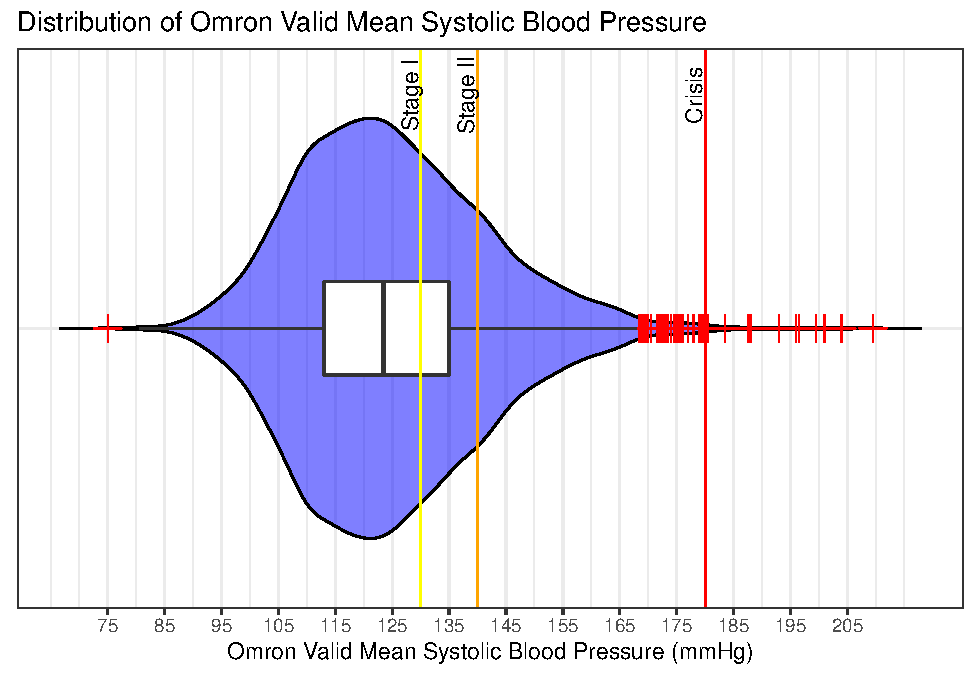
\includegraphics{figs/Outliers.pdf}

\begin{Shaded}
\begin{Highlighting}[]
\FunctionTok{par}\NormalTok{(}\AttributeTok{cex.lab=}\FloatTok{2.5}\NormalTok{)}
\FunctionTok{par}\NormalTok{(}\AttributeTok{cex.axis=}\FloatTok{2.5}\NormalTok{)}

\CommentTok{\# Basic combined violin and box plot}
\NormalTok{sd16plusA}\SpecialCharTok{$}\NormalTok{incl }\OtherTok{\textless{}{-}}\NormalTok{ haven}\SpecialCharTok{::}\FunctionTok{as\_factor}\NormalTok{(}\FunctionTok{rep}\NormalTok{(}\DecValTok{1}\NormalTok{,}\DecValTok{8204}\NormalTok{))}
\FunctionTok{ggplot}\NormalTok{(sd16plusA, }\FunctionTok{aes}\NormalTok{(}\AttributeTok{x =}\NormalTok{ incl, }\AttributeTok{y =}\NormalTok{ BMIVal)) }\SpecialCharTok{+}
  \FunctionTok{geom\_violin}\NormalTok{(}\AttributeTok{scale =} \StringTok{"width"}\NormalTok{, }\AttributeTok{trim =} \ConstantTok{FALSE}\NormalTok{, }\AttributeTok{alpha =} \FloatTok{0.5}\NormalTok{, }\AttributeTok{color =} \StringTok{"black"}\NormalTok{, }\AttributeTok{fill =} \StringTok{"blue"}\NormalTok{) }\SpecialCharTok{+}
  \FunctionTok{geom\_boxplot}\NormalTok{(}\AttributeTok{width =} \FloatTok{0.2}\NormalTok{, }\AttributeTok{fill =} \StringTok{"white"}\NormalTok{, }\AttributeTok{alpha =} \DecValTok{1}\NormalTok{, }\AttributeTok{outlier.shape =} \DecValTok{3}\NormalTok{, }\AttributeTok{outlier.colour =} \StringTok{"red"}\NormalTok{, }\AttributeTok{outlier.alpha =} \DecValTok{1}\NormalTok{, }\AttributeTok{outlier.size =} \DecValTok{4}\NormalTok{) }\SpecialCharTok{+}
  \FunctionTok{ylab}\NormalTok{(}\StringTok{"Body Mass Index (kg/m\^{}2)"}\NormalTok{) }\SpecialCharTok{+}
  \FunctionTok{ggtitle}\NormalTok{(}\StringTok{"Distribution of BMI"}\NormalTok{) }\SpecialCharTok{+}
  \FunctionTok{theme\_bw}\NormalTok{() }\SpecialCharTok{+}
  \FunctionTok{coord\_flip}\NormalTok{() }\SpecialCharTok{+}
  \FunctionTok{geom\_hline}\NormalTok{(}\AttributeTok{yintercept =} \FunctionTok{c}\NormalTok{(}\FloatTok{18.5}\NormalTok{, }\DecValTok{25}\NormalTok{, }\DecValTok{30}\NormalTok{), }\AttributeTok{colour =} \FunctionTok{c}\NormalTok{(}\StringTok{"orange"}\NormalTok{, }\StringTok{"orange"}\NormalTok{, }\StringTok{"red"}\NormalTok{), }\AttributeTok{size =} \FloatTok{0.5}\NormalTok{) }\SpecialCharTok{+}
  \FunctionTok{geom\_text}\NormalTok{(}\FunctionTok{aes}\NormalTok{(}\AttributeTok{x =} \FloatTok{1.5}\NormalTok{, }\AttributeTok{y =} \FloatTok{18.4}\NormalTok{, }\AttributeTok{label =} \StringTok{"Underweight"}\NormalTok{), }\AttributeTok{color =} \StringTok{"black"}\NormalTok{, }\AttributeTok{angle =} \DecValTok{90}\NormalTok{, }\AttributeTok{size =} \DecValTok{4}\NormalTok{) }\SpecialCharTok{+}
  \FunctionTok{geom\_text}\NormalTok{(}\FunctionTok{aes}\NormalTok{(}\AttributeTok{x =} \FloatTok{1.5}\NormalTok{, }\AttributeTok{y =} \FloatTok{24.9}\NormalTok{, }\AttributeTok{label =} \StringTok{"Overweight"}\NormalTok{), }\AttributeTok{color =} \StringTok{"black"}\NormalTok{, }\AttributeTok{angle =} \DecValTok{90}\NormalTok{, }\AttributeTok{size =} \DecValTok{4}\NormalTok{) }\SpecialCharTok{+}
  \FunctionTok{geom\_text}\NormalTok{(}\FunctionTok{aes}\NormalTok{(}\AttributeTok{x =} \FloatTok{1.5}\NormalTok{, }\AttributeTok{y =} \FloatTok{29.9}\NormalTok{, }\AttributeTok{label =} \StringTok{"Obese"}\NormalTok{), }\AttributeTok{color =} \StringTok{"black"}\NormalTok{, }\AttributeTok{angle =} \DecValTok{90}\NormalTok{, }\AttributeTok{size =} \DecValTok{4}\NormalTok{) }\SpecialCharTok{+}
  \FunctionTok{theme}\NormalTok{(}
    \AttributeTok{axis.title.y =} \FunctionTok{element\_blank}\NormalTok{(),}
    \AttributeTok{axis.text.y =} \FunctionTok{element\_blank}\NormalTok{(),}
    \AttributeTok{axis.ticks.y =} \FunctionTok{element\_blank}\NormalTok{()}
\NormalTok{  ) }\SpecialCharTok{+}
  \FunctionTok{scale\_y\_continuous}\NormalTok{(}\AttributeTok{breaks =} \FunctionTok{round}\NormalTok{(}\FunctionTok{seq}\NormalTok{(}\DecValTok{14}\NormalTok{, }\DecValTok{74}\NormalTok{, }\AttributeTok{by =} \DecValTok{5}\NormalTok{),}\DecValTok{1}\NormalTok{))}
\end{Highlighting}
\end{Shaded}

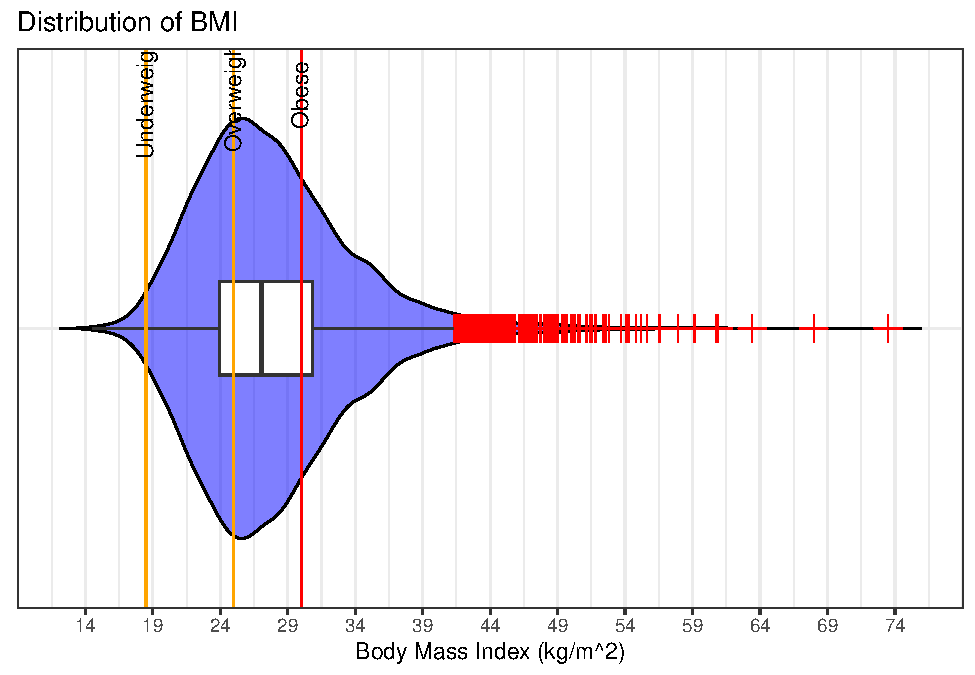
\includegraphics{figs/Outliers2.pdf}

\hypertarget{visit-based-variables}{%
\subsection{Visit-based variables}\label{visit-based-variables}}

These are not applicable for this study, as only one visit was performed
(which is the baseline, hereafter referred to as \emph{``The Nurse
Visit''}).

\hypertarget{variable-labels}{%
\subsection{Variable Labels}\label{variable-labels}}

This is less important, but I check to ensure labels are consistent,
descriptive, and limited to 40 characters.

The ``(D)'' at the start of the labels indicates that a variable was
derived, and is not a direct input from the respondent (e.g.~age bands).

\begin{Shaded}
\begin{Highlighting}[]
\FunctionTok{library}\NormalTok{(Hmisc)}

\FunctionTok{label}\NormalTok{(sd16plusA[[}\StringTok{"Age35g"}\NormalTok{]]) }\OtherTok{\textless{}{-}} \StringTok{"(D) Age, 5 year bands at 16+"}
\FunctionTok{label}\NormalTok{(sd16plusA[[}\StringTok{"wt\_int"}\NormalTok{]]) }\OtherTok{\textless{}{-}} \StringTok{"HSE2019 Weighting for analysing core interviewees"}
\FunctionTok{label}\NormalTok{(sd16plusA[[}\StringTok{"marstatD"}\NormalTok{]]) }\OtherTok{\textless{}{-}} \StringTok{"(D) Marital status incl. cohabitees"}
\FunctionTok{label}\NormalTok{(sd16plusA[[}\StringTok{"qimd19"}\NormalTok{]]) }\OtherTok{\textless{}{-}} \StringTok{"(D) 2019 IMD Quintile {-} least to most deprived"}
\FunctionTok{label}\NormalTok{(sd16plusA[[}\StringTok{"urban14b"}\NormalTok{]]) }\OtherTok{\textless{}{-}} \StringTok{"(D) Rurality of dwelling unit (urban or rural)"}
\FunctionTok{label}\NormalTok{(sd16plusA[[}\StringTok{"urban14b"}\NormalTok{]]) }\OtherTok{\textless{}{-}} \StringTok{"(D) Current use of E{-}cigarettes or vaping devices and/or NDPs"}
\FunctionTok{label}\NormalTok{(sd16plusA)}
\end{Highlighting}
\end{Shaded}

\begin{verbatim}
##                                                         SerialA 
##                              "Archive respondent serial number" 
##                                                             Sex 
##                                                              "" 
##                                                          Age35g 
##                                  "(D) Age, 5 year bands at 16+" 
##                                                          wt_int 
##             "HSE2019 Weighting for analysing core interviewees" 
##                                                        topqual2 
##                                                              "" 
##                                                        marstatD 
##                           "(D) Marital status incl. cohabitees" 
##                                                          qimd19 
##                "(D) 2019 IMD Quintile - least to most deprived" 
##                                                        urban14b 
## "(D) Current use of E-cigarettes or vaping devices and/or NDPs" 
##                                                         origin2 
##                                                              "" 
##                                                      cigsta3_19 
##                                                              "" 
##                                                      cigdyal_19 
##       "(D) Number of cigarettes smoke a day - inc. non-smokers" 
##                                                          BMIVal 
##   "(D) Valid BMI measurements using estimated weight if >130kg" 
##                                                       NDPNow_19 
##                                                              "" 
##                                                        dnoft_19 
##                                                              "" 
##                                                      drinkYN_19 
##                                                              "" 
##                                                      d7many3_19 
##         "(D) Number of days drank in last week, including none" 
##                                                        omsysval 
##                              "(D) Omron Valid Mean Systolic BP" 
##                                                            GOR1 
##                                                              "" 
##                                                            incl 
##                                                              ""
\end{verbatim}

\end{document}
